\documentclass{standalone}

\usepackage{tikz}
\usepackage{pgf-umlcd}
\usepackage[bitstream-charter]{mathdesign} % +1! taules mes petites i hi caben
\usepackage[T1]{fontenc}
\usepackage[utf8]{inputenc}

\begin{document}

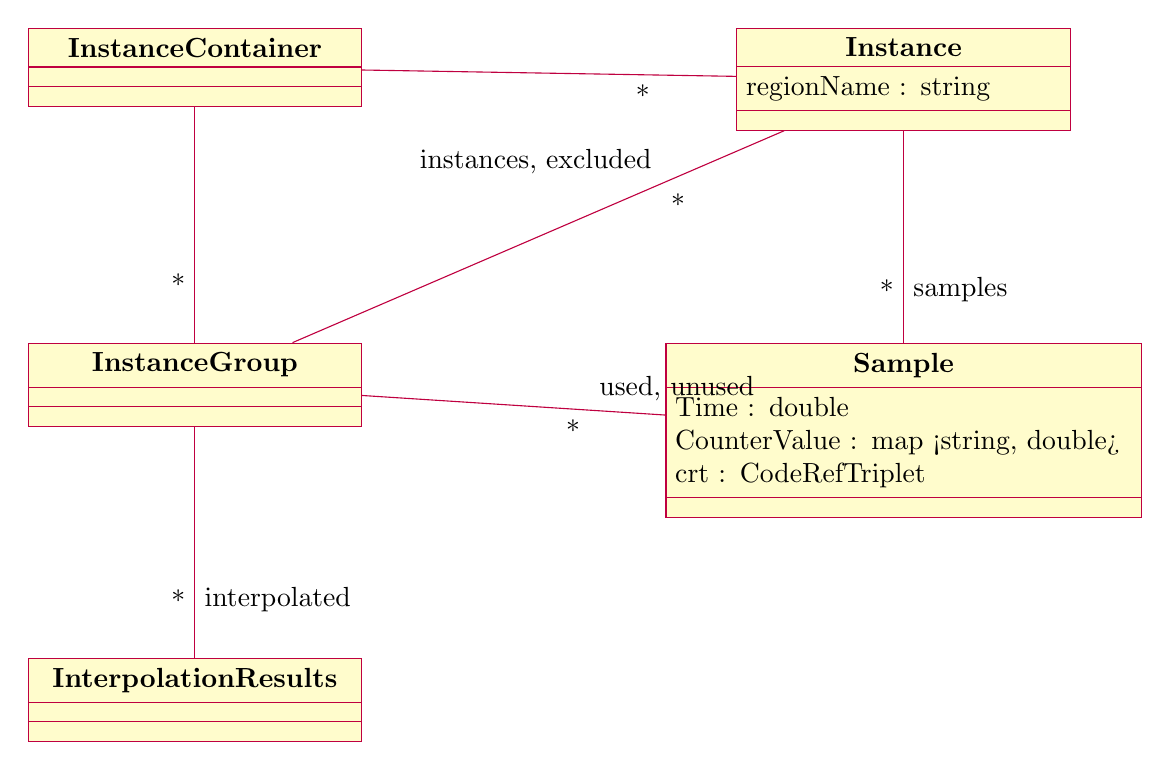
\begin{tikzpicture}

\begin{class}[text width=4cm]{InstanceContainer}{0,0}
\end{class}

\begin{class}[text width=4cm]{Instance}{9,0}
\attribute{regionName : string}
\end{class}

\begin{class}[text width=4cm]{InstanceGroup}{0,-4}
\end{class}

\begin{class}[text width=58mm]{Sample}{9,-4}
\attribute{Time : double}
\attribute{CounterValue : map <string, double>}
\attribute{crt : CodeRefTriplet}
\end{class}

\begin{class}[text width=4cm]{InterpolationResults}{0,-8}
\end{class}

\association{InstanceContainer}{}{}{Instance}{}{*}
\association{InstanceContainer}{}{}{InstanceGroup}{}{*}
\association{InstanceGroup}{}{}{Sample}{used, unused}{*}
\association{InstanceGroup}{}{}{Instance}{instances, excluded}{*}
\association{InstanceGroup}{}{}{InterpolationResults}{interpolated}{*}
\association{Instance}{}{}{Sample}{samples}{*}

\end{tikzpicture}

\end{document}
